\documentclass{article} % For LaTeX2e
\usepackage{nips14submit_e,times}
\usepackage{hyperref}
\usepackage{url}
\usepackage{graphicx}
%\documentstyle[nips14submit_09,times,art10]{article} % For LaTeX 2.09


\title{A3 homework submission \\ Team: the gurecki \\ Deep Learning 2015, Spring}


\author{
David Halpern\\
Department of Psychology\\
New York University\\
\texttt{david.halpern@nyu.edu} \\
\And
Anselm Rothe\\
Department of Psychology\\
New York University\\
\texttt{ar3918@nyu.edu} \\
\AND
Alex Rich\\
Department of Psychology\\
New York University\\
\texttt{asr443@nyu.edu} \\
}

\newcommand{\fix}{\marginpar{FIX}}
\newcommand{\new}{\marginpar{NEW}}

\nipsfinalcopy % camera-ready version

\begin{document}


\maketitle


\section{Architecture}

\subsection{Model 1}

We extended the baseline model to use Glove 100 (we couldn't solve memory errors that we got for larger Glove files).
We added a hidden layer with 500 units.

\begin{verbatim}
(1): nn.Reshape(100)
(2): nn.ReLU
(3): nn.Linear(100 -> 500)
(4): nn.Dropout
(5): nn.ReLU
(6): nn.Linear(500 -> 5)
(7): nn.LogSoftMax
\end{verbatim}



\subsection{Model 2}


\section{Learning Techniques}

Model 1 used dropout (.5). We did not invest in data augmentations. 

\section{Training Procedure}

For both models we used the typical classNLLcriterion as the loss function. We used a validation set of 13K documents (10\%) per class of the original 130K labeled training examples per class.
The optimization procedure was run over the remaining 117K (90\%) training documents per class.

\begin{figure}
	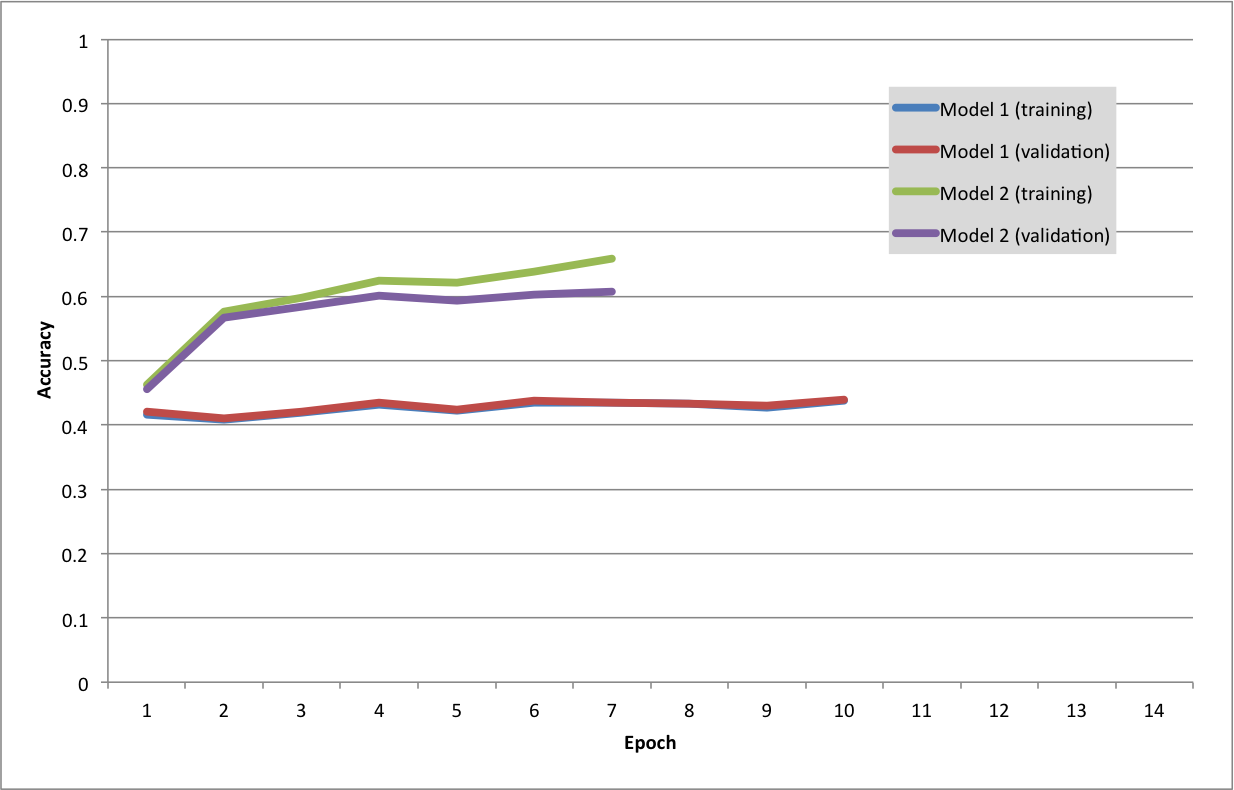
\includegraphics[width=0.8\textwidth]{Training}
\end{figure}

\subsection{Model 1}

The model was trained in 10 epochs using stochastic gradient descent with a batch size of 32, a learning rate of .1, a learning rate decay of 1e-7, a momentum of .9, and no weight decay.

\subsection{Model 2}

-- Alex


\section{Experiments}

These experiments did not help to boost the performance and thus where not included in our final submission.

\subsection{Continuous output variable}
We explored the idea that a single continuous output variable might be better than the five seperate classes because the star ratings are rank-ordered. 
For example, if the model predicts high likelihoods for class 2 and 4, then class 3 might actually be its best guess.
\begin{verbatim}
(6): nn.Linear(500 -> 4)
(7): nn.Sigmoid
(8): nn.Sum
(9): nn.Add

criterion = nn.MSECriterion()
\end{verbatim}
Layer 8 is taking the sum of 4 sigmoids which results in a number between 0 and 4 to which layer 9 adds a bias to bring the range close to 1--5.
This structure gave better results than a simple unconstrained continuous output 
\begin{verbatim}
(6): nn.Linear(500 -> 1)
\end{verbatim}
but did not reach the performance of the 5-classes output that we eventually used for Model 1.

\subsection{Phoneme understanding from scratch}
We attempted to make a model that was similar to the Crepe [2] model but rather than using characters as the features, we created a vector that used phonemic translations of the English words as features. The idea was that humans typically learn languages through sound so it is possible that the statistical dependencies of sounds would be more informative for learning than the characters themselves. If the phonemes are a nonlinear transformation of the characters that are not in the space of representations that can be learned with the standard point non-linearities and pooling operations that are often used with convolutional nets, a model using phonemes could perhaps learn better than one using just characters. In order to implement this model, we used a standard pronouncing dictionary used for NLP called CMUDict. The details of this dictionary can be found on its website: http://www.speech.cs.cmu.edu/cgi-bin/cmudict. The dictionary uses 39 standard phonemes, with 15 of these being vowels. Each vowel sound had three possible stress markers resulting in 84 possible phonemic characters. We then added a preprocessing step to translate all words in the yelp reviews that were included in the dictionary into their phonetic representations. For words that were not in the dictionary, we used the standard alphabet of lower-case english letters and punctuation markings, adding an additional 69 characters. Reviews are then represented in the same way as in the original Crepe [2] model but with a sparse vector of length 159 for each phoneme/character. While early performance was promising, we could not figure out how to deal with exploding memory/garbage collection issues in converting the reviews to phonemes and thus we could not really assess this model's performance.

\subsubsection*{References}

\small{
% [1] Dosovitskiy, A., Springenberg, J. T., Riedmiller, M., \& Brox, T. (2014). Discriminative unsupervised feature learning with convolutional neural networks. {\it Advances in Neural Information Processing Systems}, pp. 766-774.

% [2] Xiang Zhang and (2015). Text Understanding from Scratch. CoRR, abs/1502.01710, .
}


\end{document}
